\chapter{The Algorithm} \label{the_algorithm}
	In this chapter we discuss two important object detection algorithms that can classify bubbles in an image and estimate its radius. The first algorithm, which we refer to as \textit{BubbleNet} is meant to work for small bubble concentration (e.g. figure \ref{fig:aqauarium_result}) whereas the second algorithm, referred to as \textit{BubbleCurves} is better suited for bubble images with very high concentrations (figure \ref{fig:aquarium_result_high_conc}).
		
	\section{Motivation}
		We mentioned in section \ref{the_object_detection_problem} that the state of the art object detection algorithms are based on deep learning algorithms such as Faster R-CNN (cite frcnn Leute) and YOLO (Cite yolo Leute). Training these algorithms with our data (simulated and real) did not yield good results. Training a pre-trained R-CNN algorithm (i.e. transfer learning) is not meaningful either because most pre-trained models have large anchors (or rank regions boxes) and are fine tuned to work for real world photographs that contain typical objects such as humans, cars and pets. 
		
		This led us to the conclusion that such algorithms are not well suited for detecting small and dense objects (images with a low bubble concentration are also considered to have dense objects, since they contain several hundred bubble instances per image that are very close to each other). This suspicion was confirmed by (cite Zhenhua Chen et Al.) who also added that these algorithms not only rely on a large amount of training data, but also require the data to be rich in features, which does not apply to our data. 
		
	Interestingly though, scaling down anchors and training a Faster R-CNN algorithm (cite Projektpraktikum?)  from scratch did perform slightly better, with an IoU@0.5mAP of 68\%. This however, is far from ideal, so a developing a different approach was necessary to achieve better results. 
		
		
		
		
	\section{BubbleNet}\label{BubbleNet}
	
	This algorithm detects bubbles in an image with low bubble concentration and estimates their radii. The algorithm extracts candidate signals from images, classifies these signals and then computes a radius from a signal. A pseudo code is summarized in \ref{algo:bubbleNet}.
	
			\begin{algorithm}
			\begin{algorithmic}[1]
				\State \textbf{Input} Image with low bubble concentration $G$. 
				\State \textbf{Output} List of rectangles $Rec$, List of depths $Dep$
				\State Obtain local maxima $loc_max$ in $G$
				\For{Each $lm$ in $loc_max$}
					\State Extract vertical profile signal $v_p$ with length $L$.
					\If {BubbleNet($v_p$)}
						\State Compute radius $r$ and center $c$ from signal using equation \ref{eq:get_radius}
						\State Compute depth $d$ using equation \ref{eq:dof}
						\State append($Rec$, toBoundingBox($r$, $c$))
						\State append($Dep$, $d$)
					\EndIf
				\EndFor
			\end{algorithmic}
			
			\caption{BubbleNet}
			\label{algo:bubbleNet}
		\end{algorithm}
	
	\subsection{Radius from Bubble}
	
	A closer inspection of bubbles shows that a bubble can be described well by a vertical cross section going through the middle of the bubble. For instance, figure \ref{fig:bubble_profile} shows that a vertical profile is characterized by a two salient peaks: A bright peak that emerges from total reflection as explained in figure \ref{fig:bubble_physics} as well as a dimmer, yet still visible second peak at a distance $d$ from the first peak. Furthermore, simulation shows that the distance $d$ is proportional to the real bubble radius (figure \ref{fig:peaks_radius_fit}). Note that in figure \ref{fig:peaks_radius_fit} the distance $d$ was computed on rendered images, whereas the radius is a given parameter that is determined before rendering. The step wise increase in $d$ can be explained by sampling, i.e. when the radius increases by an amount smaller than a pixel, $d$ will either not change or increase by exactly 1 pixel.
	
	In order to reach a better precision, we perform a Gaussian fit around the two peaks. Here it is necessary to initialize the fit routine with reasonable values, otherwise both fits would converge towards the same function. So we first smooth the signal with a 1D Gaussian filter, and then determine the absolute maximum within the signal $m_1$ which corresponds to the first peak. The second peak corresponds to the highest local maximum $m_2$ that comes right after $m_1$. Finally, we use $arg(m_1)$ and $arg(m_2)$ as initial parameters for a Gaussian fit around the peaks. The final result is given by
	\begin{equation}
		r_{\text{measured}} = \dfrac{| \mu_1 - \mu_2 |}{2}
		\label{eq:get_radius}
	\end{equation}
	where $\mu_1$ and $\mu_2$ are the resulting parameters from the Gaussian fit that correspond the first and second peak respectively. 
	
	From previous considerations it becomes clear that a radius calibration is needed to determine the real radius from the measured radius. This is discussed in \ref{sub:radius_setup} and \ref{sub:radius_algorithm}.

		
		\begin{figure}
			\begin{subfigure}[t]{.4\textwidth}
				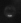
\includegraphics[scale=9]{images/one_peaks.png}
				\caption{Enlarged image of a bubble from a low concentration image. }
			\end{subfigure}
			
			\begin{subfigure}[t]{.5\textwidth}
				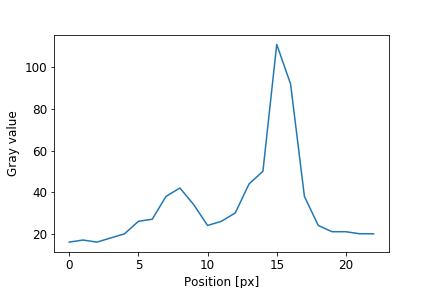
\includegraphics[scale=.5]{graphs/one_peaks_profile.png}
				\caption{Vertical bubble profile. The second peak is much dimmer than the first, but still bright enough to be distinguished from background noise.}
			\end{subfigure}
			\caption{A small air bubble from an image with low bubble concentration. }
			\label{fig:bubble_profile}
		\end{figure}
		
		\begin{figure}
			\centering
			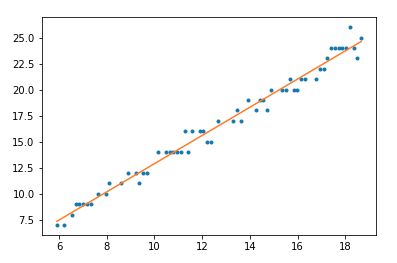
\includegraphics[scale=.7]{graphs/peak_distance_radius_fit.png}
			\caption{Simulated distance between two peaks as a function of bubble radius.}
			\label{fig:peaks_radius_fit}
		\end{figure}
	
	
	
	\subsection{Signal extraction}
		So far, we discussed how we can determine the radius from a given vertical cross section of a bubble. However, the question remains, how do we know the signal corresponds to a bubble in the first place? This is by far more challenging than determining the bubble radius and will be discussed thoroughly in the following sections. 
		
		As we can see from measurement results (section \ref{measurement_result}), extracting local maxima from an image gives good starting points for vertical profile extraction. Starting from a local maximum, we need to go a few pixels downwards $l_{d}$ to cover the whole peak and certain distance upwards $l_u$ until the second peak is reached. $l_d$ and $l_u$ are hyperparameters that add up to the total signal length $L$. The choice $l_u$ depends on the largest bubble radius that we want to detect. From (cite bubble instrument system) we know that bubbles large enough to loose their spherical shape are very rare and their contribution to gas transfer can be neglected. Also, (cite Leonie) showed that the maximum bubble diameter observed at the Aeolotron facility lies at around 500 $\mu m$ (i.e. 50 pixels). As for $l_d$, a constant value of 4 pixels is good enough to cover the large peak, because the value returned by the fit usually lies within 1 to 2 pixels away from the local maximum. 	
	
		
		\subsection{Signal classification}
		After having extracted a one dimensional signal from a potential bubble, we classify it using a convolutional neural network (CNN). 

		\subsubsection{BubbleNet architecture}		
		The architecture of our CNN is inspired from (cite Dan Li et al.), where the authors used a 1D convolutional neural network to classify electrocardiogram signals (ECG). The architecture of our CNN, called BubbleNet is shown in figure \ref{fig:cnn_arch}. 
		
		\begin{figure}
			\centering
			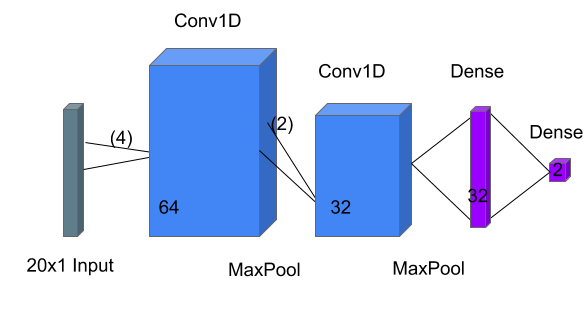
\includegraphics[scale=0.5]{images/cnn_architecture.png}
			\caption{Architecture of BubbleNet. Numbers in parentheses refer to the kernel size. The rest refers to the layer size. }
			\label{fig:cnn_arch}
			
% ########## CNN ##################
%
%		
%	   nb_classes = 2
%    nb_features = 20
%    model = Sequential()
%    model.add(Conv1D(filters=64, kernel_size=4, activation='relu', use_bias=True, input_shape=(nb_features,1)))
%    model.add(MaxPool1D(pool_size=2))
%    model.add(Conv1D(filters=32, kernel_size=2, activation='relu'))
%    model.add(Flatten())
%    model.add(Dense(32))
%    model.add(Activation('relu'))
%    model.add(Dense(nb_classes))
%    model.add(Activation('softmax'))
%		
%
%
%_________________________________________________________________
%Layer (type)                 Output Shape              Param #   
%=======================================================
%conv1d_1 (Conv1D)            (None, 17, 64)            320       
%_________________________________________________________________
%max_pooling1d_1 (MaxPooling1 (None, 8, 64)             0         
%_________________________________________________________________
%conv1d_2 (Conv1D)            (None, 7, 32)             4128      
%_________________________________________________________________
%flatten_1 (Flatten)          (None, 224)               0         
%_________________________________________________________________
%dense_1 (Dense)              (None, 32)                7200      
%_________________________________________________________________
%activation_1 (Activation)    (None, 32)                0         
%_________________________________________________________________
%dense_2 (Dense)              (None, 2)                 66        
%_________________________________________________________________
%activation_2 (Activation)    (None, 2)                 0         
%======================================================
%Total params: 11,714
%Trainable params: 11,714
%Non-trainable params: 0
		\end{figure}
		
	Note that the neural network has a fixed input size of 20 gray values. This means that resizing the vertical profiles is often necessary before passing them to the CNN. We therefore train our CNN with resized inputs in order to make robust against such preprocessing operations. 
	
	Since the bubble radius is not known prior to vertical profile extraction, we also extract $n$ signals where 
	\begin{equation}
		r_{min} \leq n \leq L
	\end{equation}
	$r_{min}$ is the smallest detectable bubble radius. It depends on the magnification factor. For the Aeolotron setup, we have $r_{min} = 90 \mu m$.

		\subsubsection{Training Data}
			The most straightforward approach to generate training data is to annotate images by hand, preferably with a precision of no less than 2 pixels. However, this can quickly become very tedious work, especially when several hundreds of thousands of images are needed to train a neural network with over $10^{3}$ parameters. Instead, we generated training data as follows:
			\begin{enumerate}
				\item Annotate 300 bubbles only by hand.
				\item Train logistic regression classifier with 300 annotated and 300 simulated images using manually computed features.
				\item Predict 100 000 bubble instances with logistic regression classifier
				\item Use data augmentation to generate a total of 200 000 vertical profiles. 				
				\item Extract 200 000 background (non bubble) images to balance data.
			\end{enumerate}
			
			For step 2, we used following features:
			\begin{itemize}
				\item First peak's gray value $p_1$
				\item Second peak's gray value $p_2$
				\item $p_1/p_2$
				\item Peaks distance $d$
			\end{itemize}
			
			The annotated images are fairly similar in size, lighting conditions and camera settings (Gamma value, gain, exposure time etc..). The reason for that, is because we want to optimize the logistic regression classifier for a high recall, regardless of its precision. So at this stage, we only want to detect as few false positives as possible, even if that means neglecting potential true positives, which in turn lower the precision. This is obviously not a good approach to classify bubbles, however, our goal at this stage is to merely generate accurately annotated data. After predicting $10^5$ true positive bubble instances from our measurements in step step 3, we processed these images further to generate more data. This included changing the gamma value, resizing (upsampling and downsampling), and vertical flipping. 
			
			Having generated more than $4 \cdot 10^5$, the neural network can now be trained. 
			
			
			
			


			
		\subsubsection{Results}
			
			We first shuffled our data and split it into training (80\%) and testing (20\%). After training for 14 epochs, the testing accuracy converged against 96.8\%, which is a very good result for a binary classifier. 
			
			For testing we used 20 more manually annotated small images, each containing from 10 to 20 bubbles. The CNN achieved IoU@0.5mAP = 91.5\% and IoU@0.3mAP = 93\%. Note that this is slightly worse than the classification accuracy result. This is due to the occasionally unprecise radius computation, which gets penalized by the IoU@p-mAP criteria. 
	
	
	
	
	
	
	
	
	
	
	
	
	
	
	\section{BubbleCurves}\label{BubbleCurves}
	\section{Calibration}\label{calibration_algorithm}
		\subsection{Depth of Field}
		\subsection{Radius}\label{sub:radius_algorithm}
